
%(BEGIN_QUESTION)
% Copyright 2006, Tony R. Kuphaldt, released under the Creative Commons Attribution License (v 1.0)
% This means you may do almost anything with this work of mine, so long as you give me proper credit

Tegn {\it bare den deriverende responsen} til en proporsjonal+deriverende regulator for følgende inngangsbetingelser, med antatt proporsjonalbånd på 250\% og derivasjonskonstant på 4 minutter. Regulatoren er {\it reversvirkende}, og algoritmen den følger er vist under grafen:

$$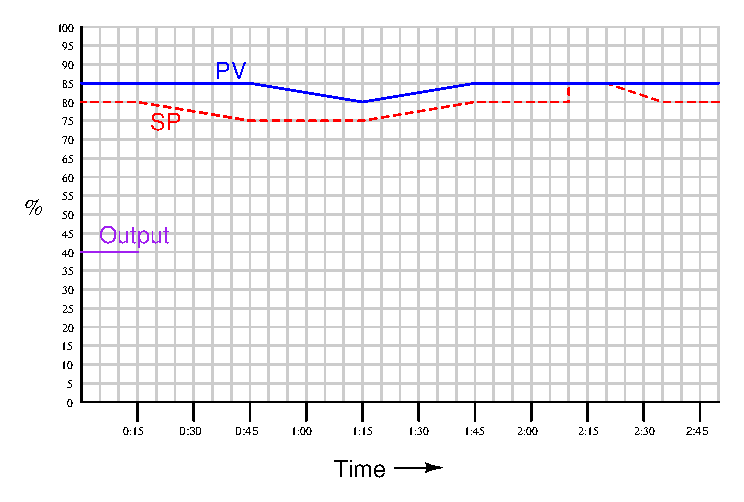
\includegraphics[width=15.5cm]{i01548x01.eps}$$

Tidsskalaen på diagrammet er minutter:sekunder, og P+D-algoritmen er som følger:

$$m = K_p \left( e + \tau_d {de \over dt} \right) + b$$

\noindent
Der,

$m$ = Regulatorutgang (manipulert variabel)

$K_p$ = Forsterkning

$e$ = Feilsignal (SP$-$PV)

$\tau_d$ = Deriverende tidskonstant

$b$ = Bias

\vskip 10pt

\underbar{file i01548}
%(END_QUESTION)





%(BEGIN_ANSWER)

$$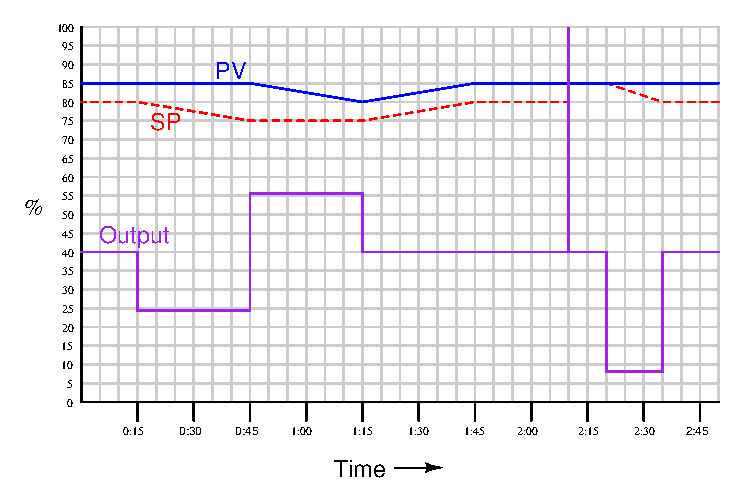
\includegraphics[width=15.5cm]{i01548x02.eps}$$

Først må vi forstå at et proporsjonalbånd på 250\% tilsvarer en forsterkning ($K_p$) på 0.4. Vi må også være klar over at siden regulatoren er reversvirkende, vil utgangen gå i samme retning som SP, men motsatt av PV.
 
\vskip 10pt

Når SP synker 5\% mellom 0:15 og 0:45, skapes en de/dt-helning på -10\% per minutt. Dette tallet, ganger $\tau_d$ = 4 og ganger $K_p$ = 0.4, gir et deriverende bidrag på -16\%. Dermed trinner utgangen ned fra 40\% til 24\% i dette tidsrommet.

Når PV synker med samme rate mellom 0:45 og 1:15, driver deriverende virkning utgangen opp med samme beløp (16\%), fra 40\% til 56\%.

Mellom 1:15 og 2:10 er det ingen endring i feilen mellom PV og SP, selv om ramping skjer mellom 1:15 og 1:45. Ved 2:15 får det positive SP-trinnet utgangen til å mette momentant på 100\%, og deretter gå tilbake til 40\%.

Fra 2:20 til 2:35 har SP en nedadgående helning på 5\%, med de/dt-rate på -20\% per minutt. Dette gir en deriverende respons på -32\%, og utgangen trinner ned fra 40\% til 8\%. Ved tid 2:35, når SP slutter å rampe, opphører den deriverende virkningen og utgangen returnerer til 40\%.

%(END_ANSWER)





%(BEGIN_NOTES)


%INDEX% Control, proportional + derivative: graphing controller response

%(END_NOTES)

